
\section{Introduction} \label{sec:introduction}

Many robotic applications, especially those that involve human robot interaction, often require a rich representation of the environment in order to perform such behavior as path planning and obstacle avoidance. In general, a rich representation, or map, is useful for providing situational awareness to an autonomous agent. A map is also important for applications such as teleoperation \cite{Kadous2006}.

The methodology to build this
representation is a continuously evolving subject in the field of robotics.
The origins of the research into this problem dates back roughly 25 years \cite{Lorensen1987}.
Since then the methods and the representations themselves have continued to
evolve at an impressive rate. The main catalyst behind this growth is the
advancement of sensing technologies over the same time period. In general,
sensors have continued to generate measurements at higher rates, higher
resolution, and lower cost over the years. This has provided an amazing
opportunity to build richer and more useful representations of the
environment.

In robotics map building in an unknown environment is referred to as
the Simultaneous Localization and Mapping (SLAM) problem \cite{Thrun2002}. This label
describes the fact that a methodology which solves the SLAM problem must
simultaneously locate the robot in the environment as well as map the
environment.

The focus of this work is the mapping aspect of the SLAM problem.
Early mapping methods represented
the environment as a set of landmark locations. The result was a sparse set
of points usually on a 2D plane. This allowed research to show that their
SLAM solutions worked but it soon became clear that a richer representation
of the world was needed for a growing number of applications. In response
several methods were developed using various other representations.  A
number of representations are compared in Table \ref{tab:rep}.

\begin{table}[h]
\begin{footnotesize}
\begin{center}
\begin{tabular}{|l|c|c|c|c|c|}
\hline
\multirow{2}{*}{} & Adaptability & Computationally & Low Memory & SA: & SA: \\
 & & Inexpensive & Requirement & Robot & Human \\\hline
Landmark Locations  	& x & x & x & - & - \\
Point Clouds		& - & x & - & - & - \\
Surfels             	& x & x & x & - & x \\
Implicit Functions 	& x & - & - & x & x \\
Static Mesh	 	& - & x & x & x & x \\
Adaptive Mesh	 	& x & o & o & x & x \\
\hline
\end{tabular}
\end{center}
\end{footnotesize}
\caption{Characteristics of current forms of representation}
\label{tab:rep}
\end{table}

Table \ref{tab:rep} compares the characteristics of map the
representations. Adaptability describes the ability of the representation
to correct itself given new information. Computational expense describes
how difficult it is to create and maintain a representation.  Memory
requirement describes how much memory a method must use to run.  Situation
Awareness (SA) describes how well suited a representation is for both robot
and human decision making. Robot decision making requires a representation
that can be used for such problems as obstacle avoidance. Human decision
making requires a method that can be allow an operator to intuitively
understand the state of the robot given the map. The Table is supposed to
reflect what a representation is capable of and not necessarily where the
state-of-the-art is.

A mesh based representation is arguably an extremely good choice in
comparison to the other representations. It has been used extensively by
the gaming community because it is the best for representing large
environments with the minimum memory. Also, this sort of representation
works well to increase the SA of a robot because methods for performing
physical simulations such as obstacle collision detection already exist. In
addition, a mesh based environment is a very natural method to display
information to a human operator.

Currently, the problem with mesh-based environmental mapping techniques is
that they are greedy in the sense that the mesh elements can not be
corrected using new information. Once the mesh is in place there is no
mechanism to adapt to newer measurements. The problem of adapting a mesh to
new information is a very well studied problem in computer graphics, but
these methods were not designed with large scale environmental mapping in
mind. The biggest questions are:

\begin{itemize}
\item How can we quickly decide which measurements should be used to adapt
which part of the mesh?
\item How can we quickly detect new and removed objects?
\item How can we robustly deal with noise and obtain a methodology that makes use of the new
measurements of an already existing part of the representation?
\end{itemize}

So the real question is can we develop a methodology that can address all
of the above questions and still have a manageable memory requirement and
be computationally feasible? The goal of this work is to show that MABDI is
capable of addressing these questions.

\begin{figure}[thpb]
\centering
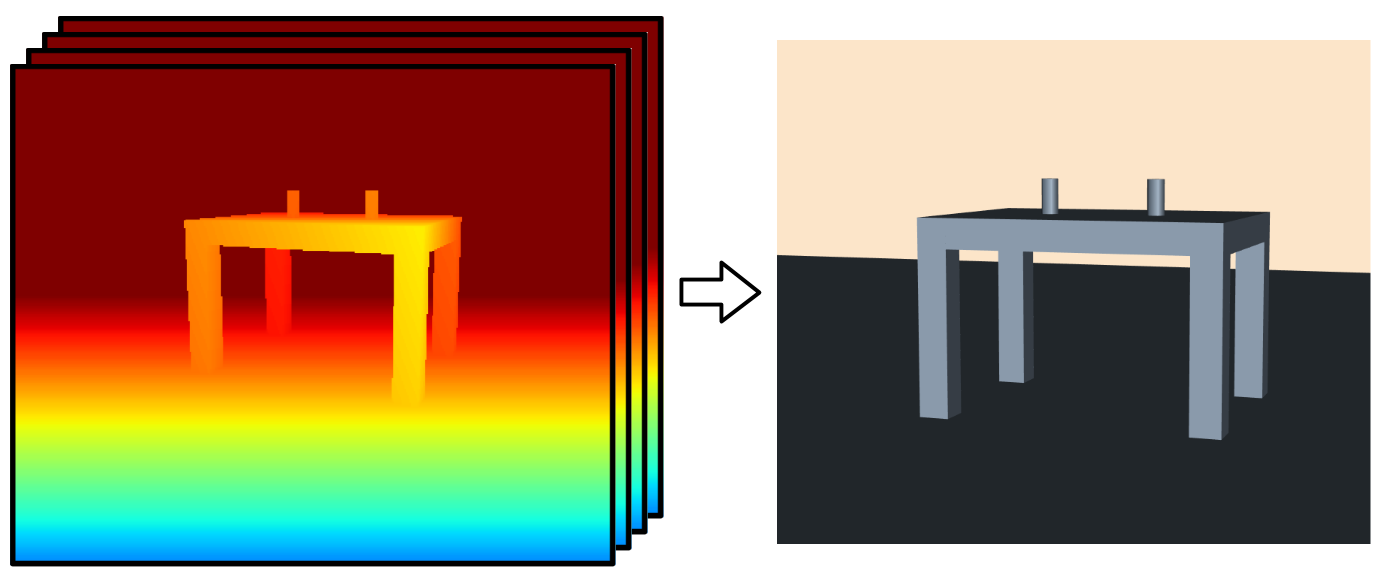
\includegraphics[width=.5\textwidth]{figures/diagram_goal.png}
\caption{In this work, the goal of mapping is to generate  }
\label{fig:goal}
\end{figure}
